\section{Durchführung}
\label{sec:Durchführung}

Ein schematischer Aufbau ist in Abbildung \ref{fig:Aufbau} dargestellt. 

\begin{figure}
  \centering
  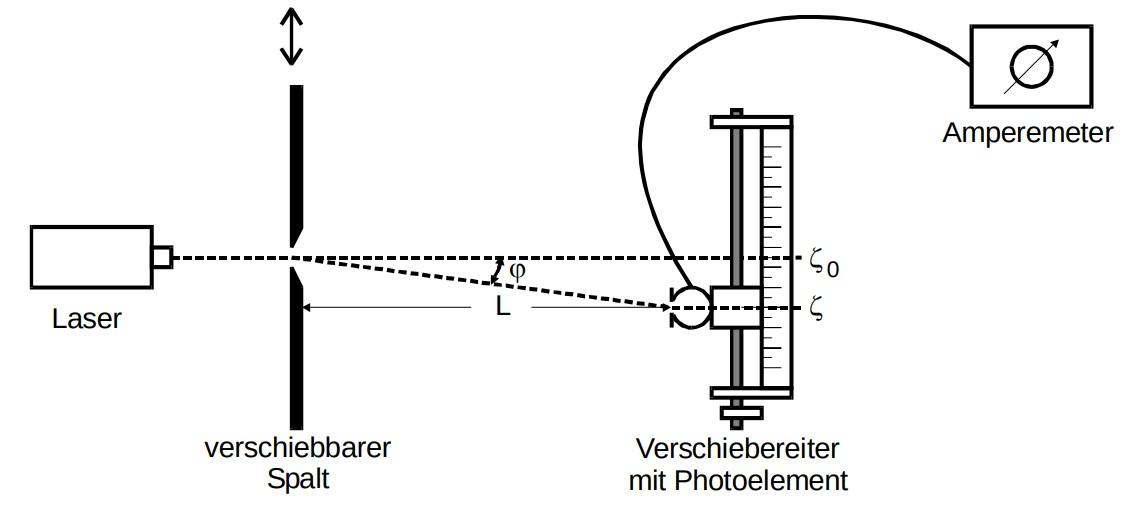
\includegraphics[scale=0.3]{content/Aufbau.jpg}
  \caption{Versuchsanordnung zur Abmessung einer Beugungsfigur. [1]}
  \label{fig:Aufbau}
\end{figure}

Zunächst wird die Strecke $L$ ausgemessen, die den Abstand zwischen dem Spalt und dem Photoelement angibt. 
Anschließend wird der erste Einzelspalt untersucht. Es ist darauf zu achten, dass vor jeder Messung 
bereits ein Strom $I_\text{Dunkel}$ gemessen werden muss, da das Photoelement auch im wenig beleuchteten 
Zustand eine Intensität wahrnimmt. Dazu wird zunächst der Photostrom ohne angeschalteten Laser gemessen 
und der Offset $I_\text{Dunkel}$ notiert. 
Für die eigentliche Intensitätsmessung wird der Gegenstand wieder entfernt und der angezeigte Strom $I$ notiert. \\
Das Photoelement wird nach diesen beiden Messungen weiter verschoben und die nächsten Messungen werden 
durchgeführt. In der Nähe des Hauptmaximums wird das Photoelement in $\SI{0.25}{\milli\meter}$ Schritten bewegt, weiter 
außen in $\SI{0.5}{\milli\meter}$ bzw. $\SI{1}{\milli\meter}$ Schritten. Aus dieser Messung ergeben sich insgesamt 
Datenpaare bestehend aus der Verschiebung $x$ des Photoelements und $I$. \\
Insgesamt wird das Photoelement in beide Richtung des Hauptmaximas um $\SI{25}{\milli\meter}$ verschoben. \\
Der zweite Einzelspalt und der Doppelspalt werden analog vermessen. \\
Als letzter Schritt werden die tatsächlichen Spaltbreiten und Abstände der Spalte notiert. 
